\documentclass[xcolor=svgnames, usepdftitle=false, aspectratio=169]{beamer}
\usepackage{pgfpages}
\setbeameroption{hide notes}

\frenchspacing

% --- THEME ---
\usetheme[progressbar=frametitle]{metropolis}

\useoutertheme{metropolis}
\useinnertheme{metropolis}
\usefonttheme{metropolis}
\usecolortheme{dove}  % spruce, metropolis, dove, crane, beaver, seagull
\setbeamercolor{background canvas}{bg=transparent}
\usecolortheme[named=DarkOrange]{structure}
\usefonttheme[onlymath]{serif}

% \setbeamersize{text margin left=5.03cm}
\setbeamercolor{title separator}{fg=DarkOrange}

% --- HACKS ---
% Hide numbers on standout slides.
\setbeamertemplate{frame numbering}{
    \ifbool{metropolis@standout}{}{
        \insertframenumber
    }
}
\setbeamertemplate{frame numbering}[counter]  % none, counter, fraction

% Avoid font-warning with itemize bullets.
\renewcommand\textbullet{\ensuremath{\bullet}}

% --- PACKAGES ---
\usepackage[UKenglish]{babel}
\usepackage[utf8]{inputenc}
\usepackage{lmodern}
\usepackage[T1]{fontenc}

% \usepackage{appendixnumberbeamer}
\usepackage{upquote}
\usepackage[straightquotes]{newtxtt}
\usetikzlibrary{positioning}
% \usepackage{minted}
\usepackage{multicol}
\usepackage{xspace}
\usepackage{booktabs}
\usepackage{siunitx}

% --- SETTINGS ---
\graphicspath{{../figures/}}
\setlength{\fboxsep}{0pt}

% --- OWN COMMANDS ---
\newcommand{\bdra}{\ensuremath{\boldsymbol \Rightarrow }~}
\newcommand{\bdla}{\ensuremath{\boldsymbol \Leftarrow }~}
\newcommand{\dra}{\ensuremath{\Rightarrow }~}
\newcommand{\dla}{\ensuremath{\Leftarrow }~}
\newcommand{\mr}[1]{\mathrm{#1}}
\newcommand{\emg}[2]{\texttt{emg#1#2}\xspace}
\newcommand{\empymod}{\texttt{empymod}\xspace}
\newcommand{\ohmm}{\ensuremath{\Omega\,}\text{m}\xspace}
\newcommand{\rmk}[1]{{\color{red}\bfseries #1}}
\newcommand{\maybe}[1]{{\color{gray} #1}}
\newcommand{\todo}{{\color{red}\texttt{TODO:}}\xspace}
\newcommand{\bm}[1]{{\mathbf{#1}}}

% --- TITLE-STUFF ---

\newcommand{\ttitle}{Time-domain CSEM modelling}
\title{\vspace{2.5cm}\color{white}{\ttitle}}
\subtitle{\color{white}{using frequency- and Laplace-domain computations}}
\date{\color{white}{20 October 2021}}
\author{\vspace{-.3cm}\color{white}{Dieter Werthmüller and Evert Slob, TU Delft}}
\institute{}

\hypersetup{pdftitle={\ttitle}, allcolors=NavyBlue, colorlinks=true}

% --- SLIDES ---
\begin{document}
\metroset{block=fill}  % Fills the block-environment
\usebackgroundtemplate{
\includegraphics[width=\paperwidth]{SlideTitle}}

\maketitle % ---------------------------------------------------------------- %
\usebackgroundtemplate{
\includegraphics[width=\paperwidth]{SlideContent}}

\begin{frame}
  {Time-domain modelling with a frequency-domain code}
  \centering

  \bdra \quad (1) Frequency selection \quad (2) Gridding \quad \bdla\\[.5cm]

  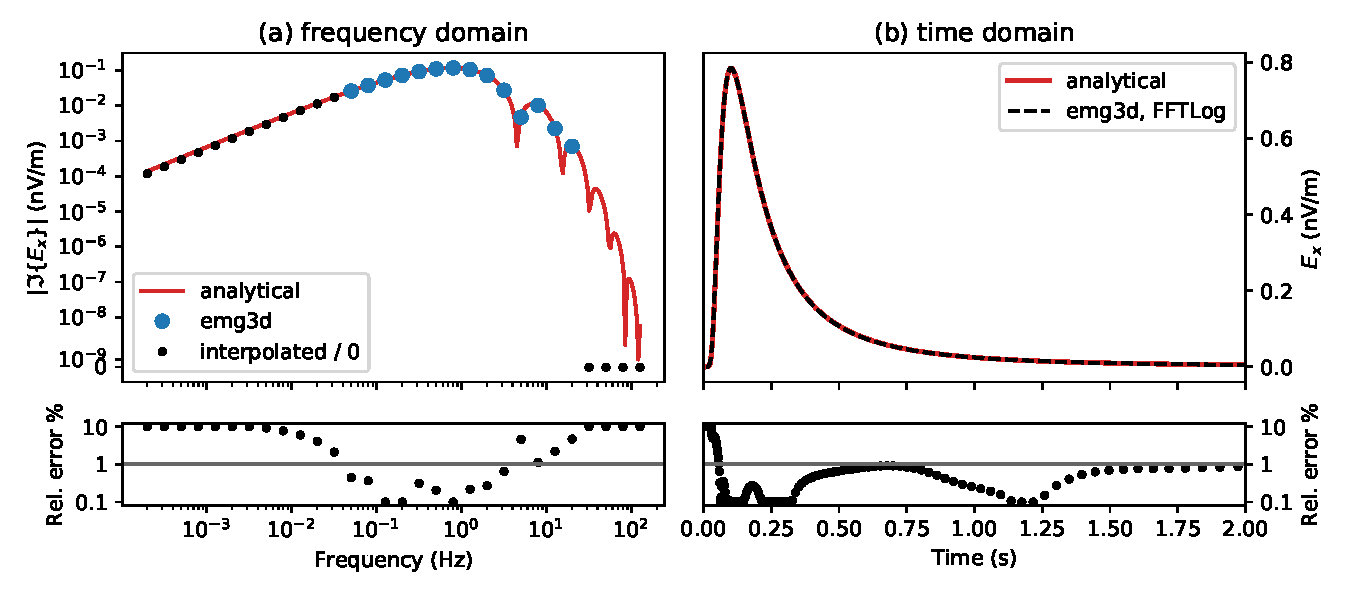
\includegraphics[width=.8\textwidth]{fullspace}


  {\raggedright\small
  Werthmüller et al., 2021, \emph{Fast Fourier transform of electromagnetic
  data\\for computationally expensive kernels}, GJI; DOI:
  \href{https://doi.org/10.1093/gji/ggab171}{10.1093/gji/ggab171}.\\
  }


\end{frame}

\begin{frame}
  {Laplace-domain computation}
  \centering
  \vspace{-.5cm}

  % Correct for: e^+iwt: + s σ E − ∇ × µ^-1 ∇ × E = − s J
  %              e^-iwt: + s σ E + ∇ × µ^-1 ∇ × E = − s J
  $$
    \mr{i}\omega \rightarrow s:
    \qquad
    \textcolor{red}{s} \sigma \mathbf{E} \ +\
    \nabla \times \mu^{-1} \nabla \times \mathbf{E}
    \ =\ -\textcolor{red}{s} \mathbf{J}_\mathrm{s}
  $$

  \bdra Faster\quad (1) Computation\quad (2) Convergence \quad \bdla\\
  \vspace{.5cm}

  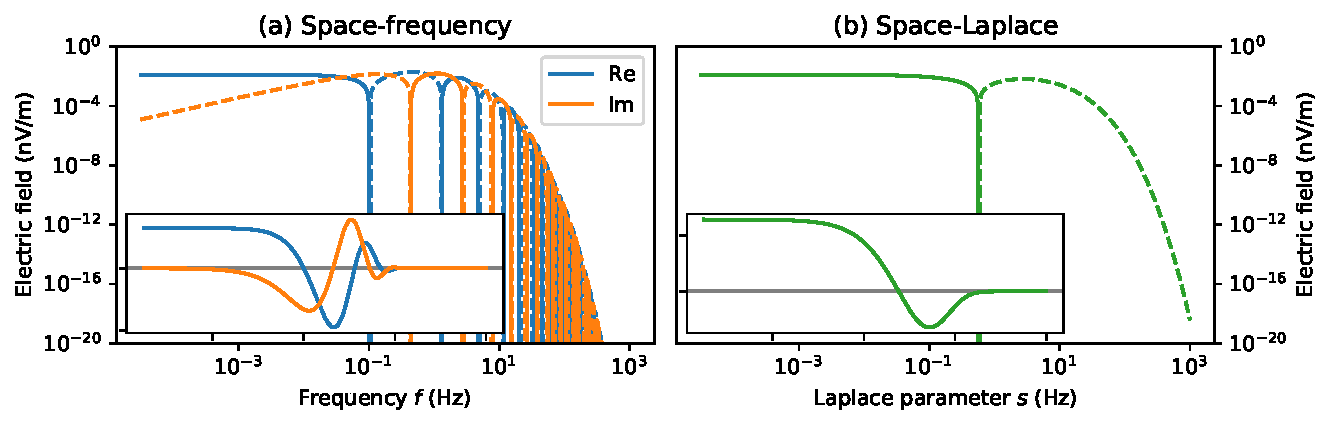
\includegraphics[width=\textwidth]{motivationcomparison}

\end{frame}

\begin{frame}
  {Laplace-to-time domain transformations}

  \begin{enumerate}
    \item Design digital linear filters for the transform
    \item Carry out transform for semi-analytical (layered) responses
    \item Test stability
  \end{enumerate}


  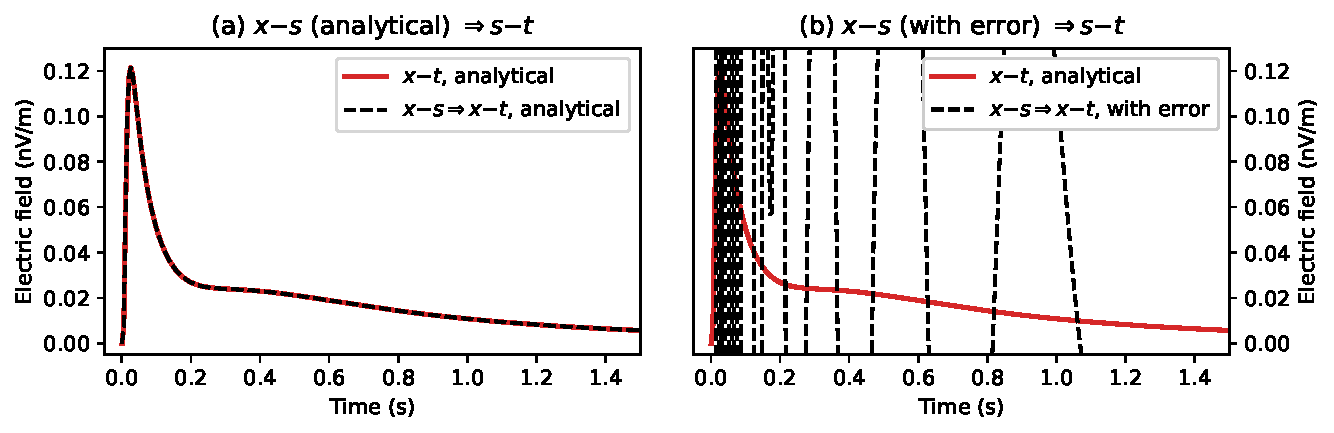
\includegraphics[width=\linewidth]{s-t_time}%

\end{frame}

\begin{frame}
  {ePoster -- Outlook}

  \begin{itemize}\itemsep.5cm
    \item Time-domain modelling with a frequency-domain code:\\
      15--25 frequencies are usually enough
    \item Laplace-domain computation
    \item Laplace-to-time domain transformation
    \item Laplace-to-frequency domain transformation
  \end{itemize}

  \vspace{.5cm}

  Used open-source codes:\\
  \empymod (layered models) \& \emg3d (3D models), see
  \href{https://emsig.xyz}{emsig.xyz}.

\end{frame}

\end{document}
